\newpage
\subsection{Software Work}

% Give a brief software overview
%\textbf{Software Brief: }
\subsubsection{Software Brief: }
RIMA1 and RIMA2 run off the ROS1 Melodic framework. They utilised custom messages and customised ROS packages to function. All code for the robot was written in C++ and analysis scripts used for PEC are written
in Python. Unfortunately the codebases for these robots cannot be shared as it is property of UTS and Sydney Water. The robots processes and GUI's are all run/launched using shell scripts in the linux CL.

% New RIMA1 system board software update
\vspace{\baselineskip}
%\textbf{RIMA1 System Board Software Update: }
\subsubsection{RIMA1 System Board Software Update: }
The new system board required some minor software updates. This primarily consisted of changes to message data types and names. This change also required small modification to RIMA1's core.cpp file which was responsible 
for ROS handling (i.e. setting up subscribers, publishers, etc.). 

% RIMA1 GUI Update
\vspace{\baselineskip}
%\textbf{RIMA1 GUI Update: }
\subsubsection{RIMA1 GUI Update: }
The old GUI of RIMA was outdated and not greatly designed and doing something simple such as turning required going into settings and modifying rotation setpoints which is clearly not ideal or user friendly. I updated
the GUI [~\ref{fig:r1gui}] to have more intuitive control, I also installed rear cameras at the time for rear view and visual view of the sensor to have a better cue of full expansion rather than basing it off the current reading. Basic 
IMU visualisation was also added to the GUI to allow for better understanding of the robot's orientation in the pipe. The GUI was written in C++ using Qt Designer.

\begin{figure*}[htbp]
    \centering
    \subfloat[Old RIMA1 interface]{
        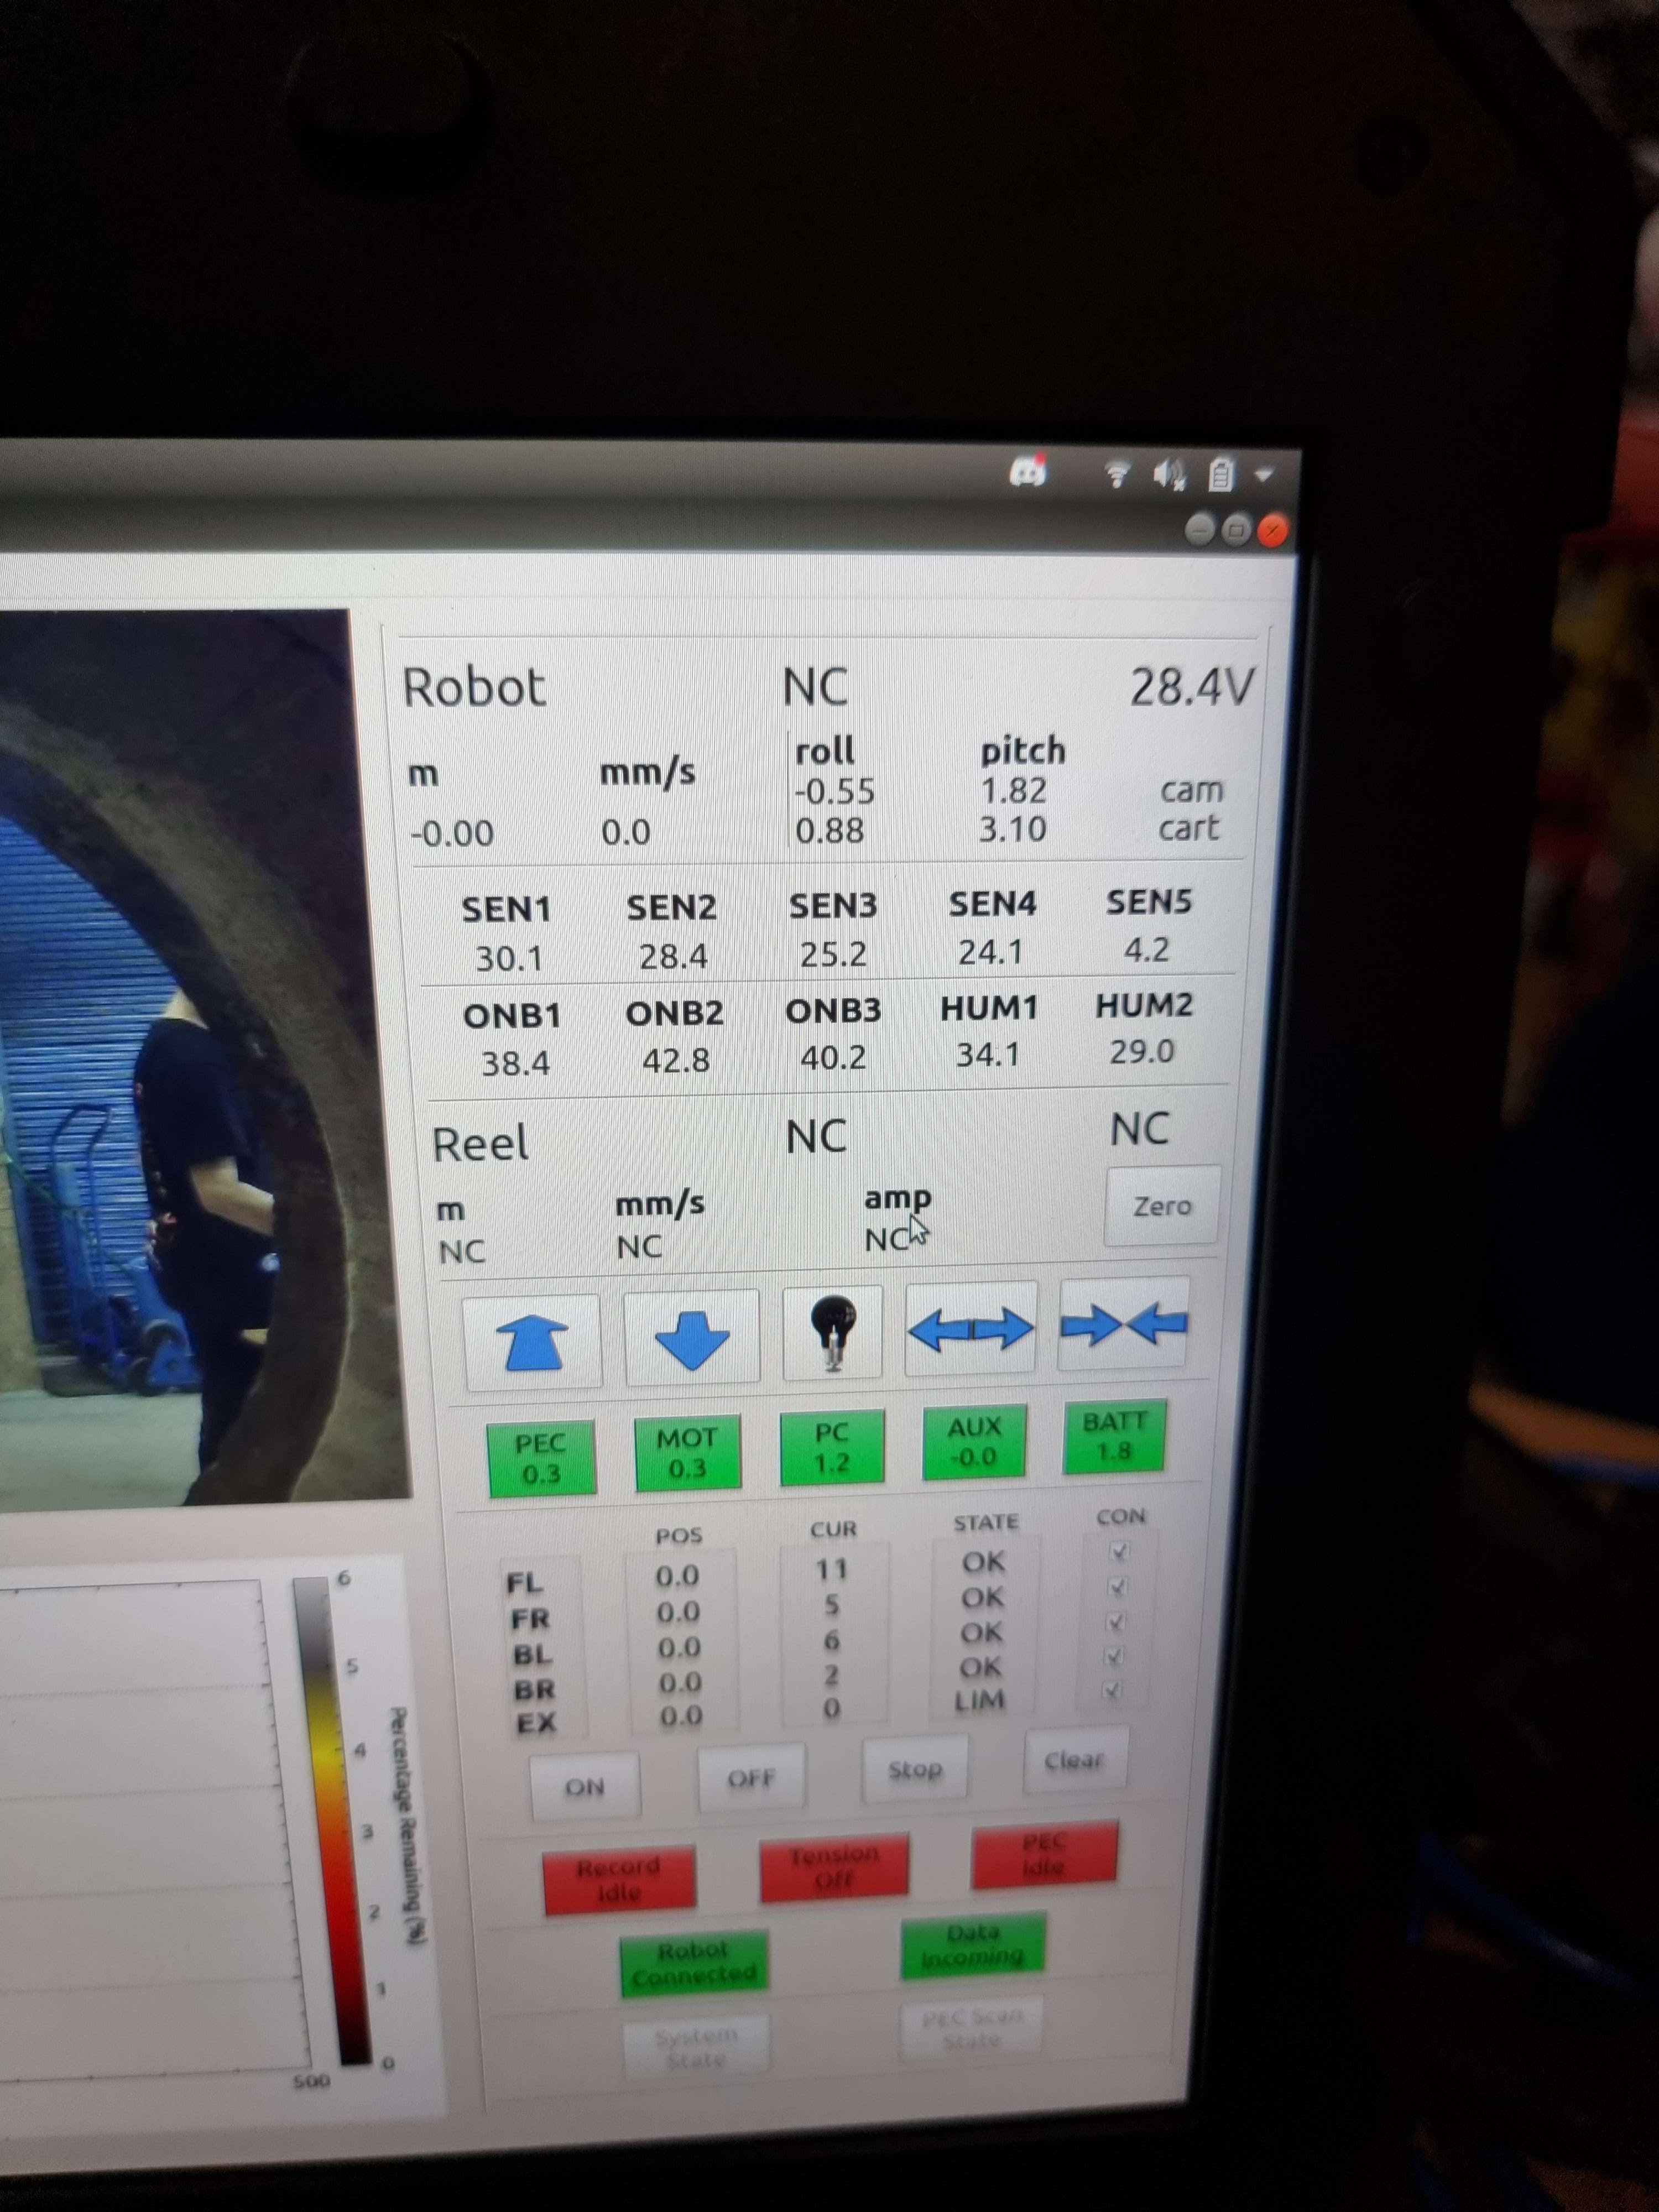
\includegraphics[width=0.30\textwidth, valign=c]{images/rima1/rima1_old_gui.jpg}
    }
    \hspace{0.5cm}
    \subfloat[New RIMA1 interface]{
        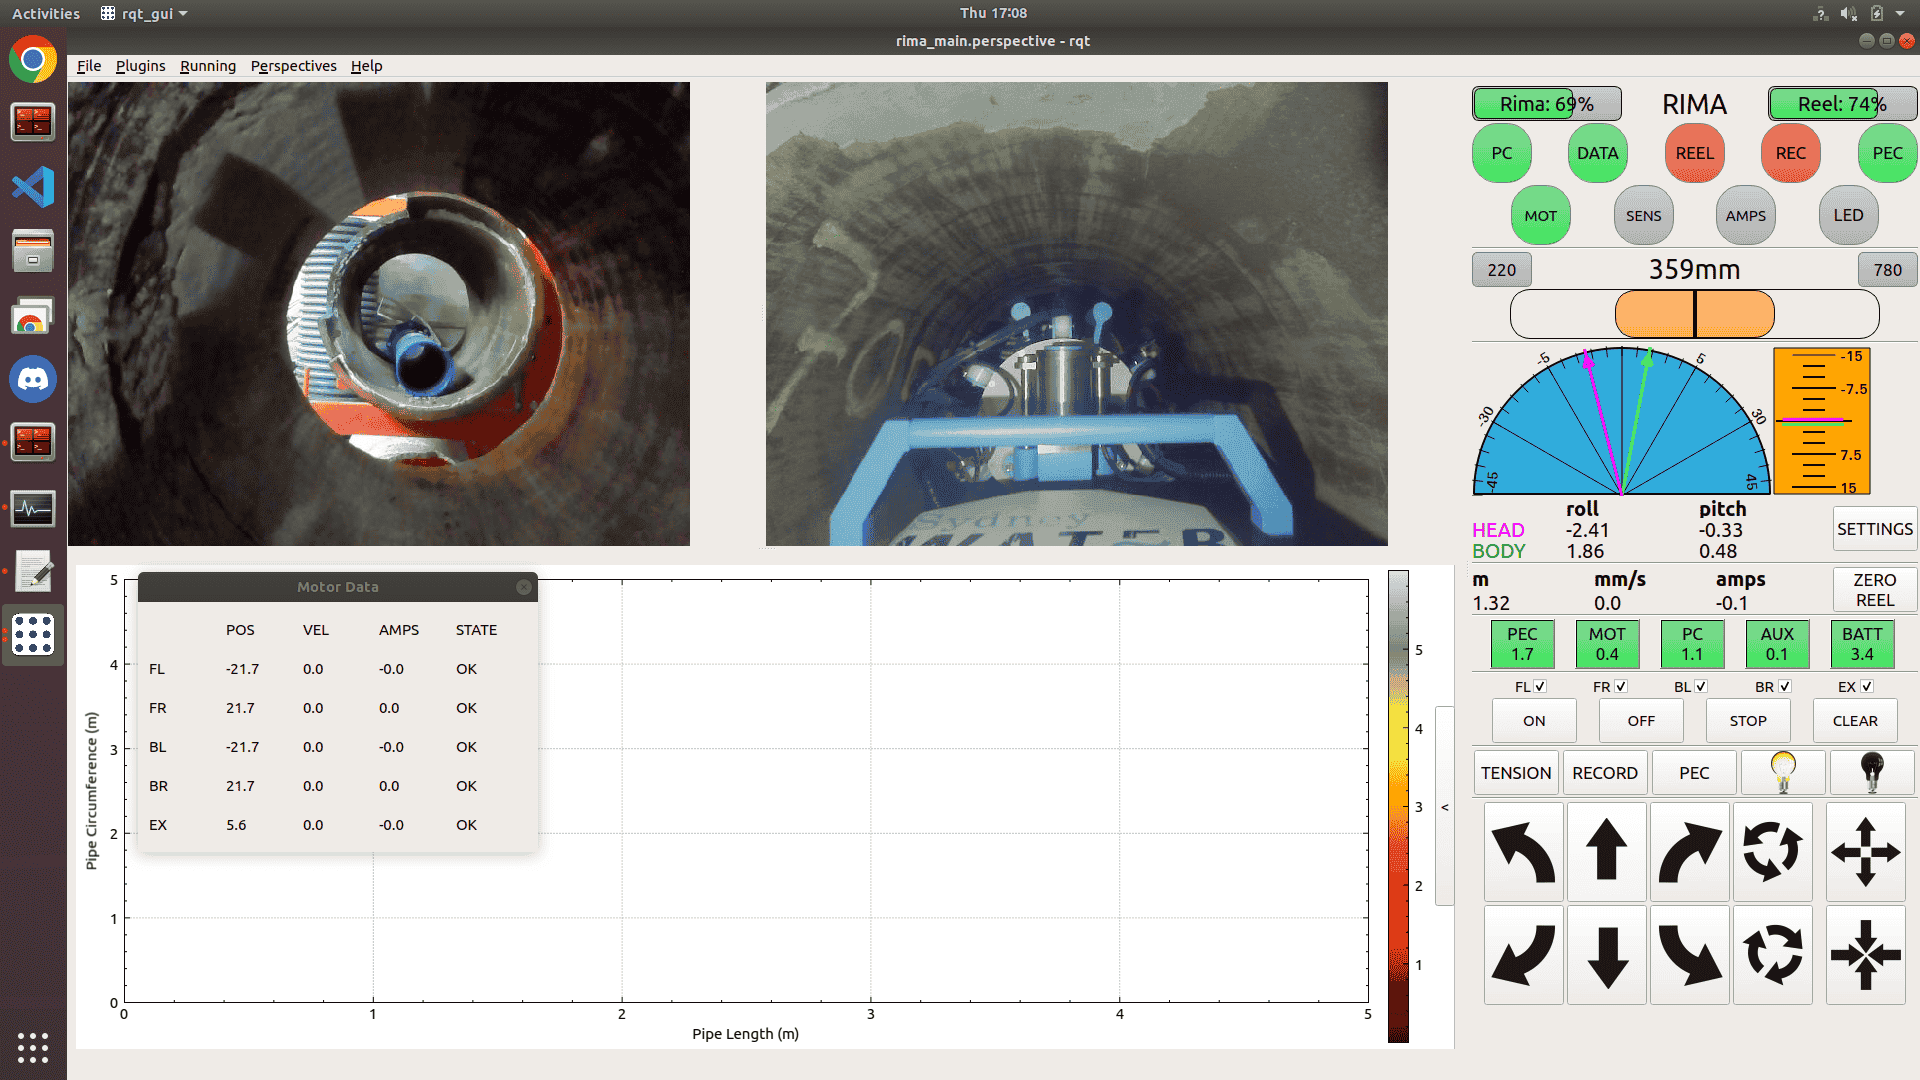
\includegraphics[width=0.60\textwidth, valign=c]{images/rima1/rima_gui_new.png}
    }
    \caption{Comparison of RIMA1 GUI's}
    \label{fig:r1gui}
\end{figure*}
\newpage
\imginin{rima1/rear_cam_rear.jpg}{RIMA1 Rear Camera rear View}{rcam}{0.8}

% Embedded software debugging for RIMA2 PEC
\subsubsection{RIMA2 PEC Embedded Software Debugging: }

When RIMA2's PEC Board was installed, its microcontroller onboard the PCB was also upgraded and used slightly different libraries compared to the old PCB for SPI communication. The Sensor Head has 10 PEC
channels that each have an ADC which are daisy-chained together. From a software standpoint the channels buffer through in a loop so all 10 channels are obtained and transferred via SPI. With the new MCU, Libary and PEC board,
10 inidvidual channels of data did not come through. Instead the 1st channel appeared to override all channels and there were 10 identical plots of data. After logic analysing and electrical debugging, if was found that 
the Chip Select was a consant (set this way in the updated library) and as a result, would not allow proper buffering through the ADCs. Once this was changed, PEC worked as expected.

% PEC Calibration
\newpage
\subsubsection{RIMA PEC Calibration: }
PEC was regularly calibrated before field trials to ensure that sensors were fully functional. PEC curves could be extracted and analysed [~\ref{fig:pecdata1}] [~\ref{fig:pecdata2}] using Python Scripts. 

\imginin{rima1/lo_0mm_th_all.png}{PEC data RIMA2 no concrete lining results}{pecdata1}{0.58}
\imginin{rima1/lo_11.54mm_th_all.png}{PEC data RIMA2 11.54mm concrete lining results}{pecdata2}{0.58}

% Simplified shell script for data tranfer and other stuff
\newpage
\subsubsection{Other Software Work:}

There were a few other software tasks I did such as creating new shell scripts for QOL such as easier data transfer between robot and base station. This made it more intuitve for anyone using to command line rather than having to memorise
various terminal commands. I was also in the process of creating a Master GUI in collaboration with our Senior Engineer. This was to make everything more user firendly for Sydney Water to grant them capability in having non-technical
staff operate the robots. However, due to project timeline constraints, whilst built, it was never tested fully.
